% DO NOT COMPILE THIS FILE DIRECTLY!
% This is included by the other .tex files.

\begin{frame}[t,plain]
\titlepage
\end{frame}

\begin{frame}
\frametitle{From Tagging to Flexible Taxonomies}
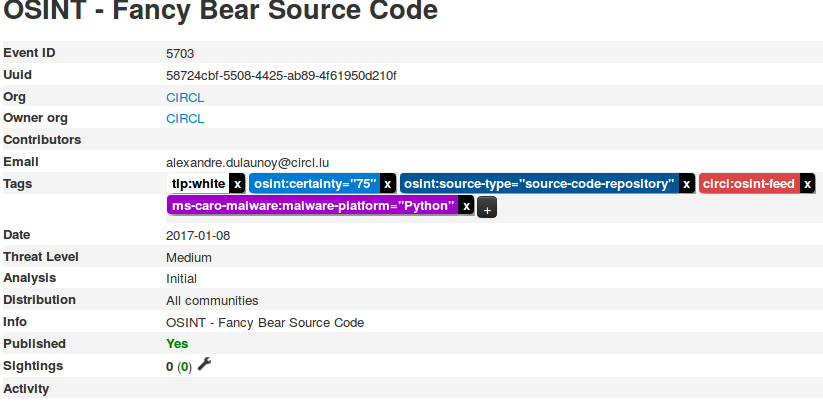
\includegraphics[scale=0.3]{tags.png}
\begin{itemize}
   \item Tagging is a simple way to attach a classification to an event or an attribute.
   \item In the early version of MISP, tagging was local to an instance.
   \item {\bf Classification must be globally used to be efficient}.
   \item After evaluating different solutions of classification, we built a new scheme using the concept of machine tags.
\end{itemize}
\end{frame}

\begin{frame}
\frametitle{Machine Tags}
        \begin{itemize}
                \item Triple tag, or machine tag, format was introduced in 2004 to extend geotagging on images.
        \end{itemize}
        {
                \setlength{\fboxsep}{1pt}
                \setlength{\fboxrule}{1pt}
                \fbox{
\includegraphics[scale=0.7]{machinetag.pdf}}
        }
        \begin{itemize}
        \item A machine tag is just a tag expressed in way that allows systems to parse and interpret it.
        \item Still have a human-readable version:\\
        \begin{itemize}
                \item admiralty-scale:source-reliability="Fairly reliable"
        \end{itemize}
        \end{itemize}
\end{frame}

\begin{frame}
\frametitle{MISP Taxonomies}
\begin{itemize}
\item Taxonomies are implemented in a simple JSON format.
\item Anyone can create their own taxonomy or reuse an existing one.
\item The taxonomies are in an independent git repository\footnote{\url{https://www.github.com/MISP/misp-taxonomies/}}.
\item These can be freely reused and integrated into other threat intel tools.
\item Taxonomies are licensed under Creative Commons (public domain) except if the taxonomy author decided to use another license.
\end{itemize}
\end{frame}

\begin{frame}
\frametitle{Existing Taxonomies}
\begin{itemize}
\item NATO - {\bf Admiralty Scale}
\item CIRCL Taxonomy - {\bf Schemes of Classification in Incident Response and Detection}
\item eCSIRT and IntelMQ incident classification
\item EUCI {\bf EU classified information marking}
\item Information Security Marking Metadata from DNI (Director of National Intelligence - US)
\item NATO Classification Marking
\item OSINT {\bf Open Source Intelligence - Classification}
\item TLP - {\bf Traffic Light Protocol}
\item Vocabulary for Event Recording and Incident Sharing - {\bf VERIS}
\item And many more like ENISA, Europol, or the draft FIRST SIG Information Exchange Policy.
\end{itemize}
\end{frame}

\colorlet{punct}{red!60!black}
\definecolor{background}{HTML}{EEEEEE}
\definecolor{delim}{RGB}{20,105,176}
\colorlet{numb}{magenta!60!black}
\lstdefinelanguage{json}{
    basicstyle=\scriptsize,
    numbers=left,
    numberstyle=\scriptsize,
    stepnumber=1,
    numbersep=5pt,
    showstringspaces=false,
    breaklines=true,
    frame=lines,
    backgroundcolor=\color{background},
    literate=
     *{0}{{{\color{numb}0}}}{1}
      {1}{{{\color{numb}1}}}{1}
      {2}{{{\color{numb}2}}}{1}
      {3}{{{\color{numb}3}}}{1}
      {4}{{{\color{numb}4}}}{1}
      {5}{{{\color{numb}5}}}{1}
      {6}{{{\color{numb}6}}}{1}
      {7}{{{\color{numb}7}}}{1}
      {8}{{{\color{numb}8}}}{1}
      {9}{{{\color{numb}9}}}{1}
      {:}{{{\color{punct}{:}}}}{1}
      {,}{{{\color{punct}{,}}}}{1}
      {\{}{{{\color{delim}{\{}}}}{1}
      {\}}{{{\color{delim}{\}}}}}{1}
      {[}{{{\color{delim}{[}}}}{1}
      {]}{{{\color{delim}{]}}}}{1},
}

\begin{frame}[fragile]
\frametitle{Want to write your own taxonomy? 1/2}
\begin{lstlisting}[language=json,firstnumber=1]
{
  "namespace": "admiralty-scale",
  "description": "The Admiralty Scale (also called the NATO System) is used to rank the reliability of a source and the credibility of an information.",
  "version": 1,
  "predicates": [
    {
      "value": "source-reliability",
      "expanded": "Source Reliability"
    },
    {
      "value": "information-credibility",
      "expanded": "Information Credibility"
    }
  ],
....
\end{lstlisting}
\end{frame}

\begin{frame}[fragile]
\frametitle{Want to write your own taxonomy? 2/2}
\begin{lstlisting}[language=json,firstnumber=1]
{
  "values": [
    {
      "predicate": "source-reliability",
      "entry": [
        {
          "value": "a",
          "expanded": "Completely reliable"
        },
....
\end{lstlisting}
\begin{itemize}
        \item Publishing your taxonomy is as easy as a simple git pull request on misp-taxonomies\footnote{\url{https://github.com/MISP/misp-taxonomies}}.
\end{itemize}
\end{frame}

\begin{frame}
\frametitle{How are taxonomies integrated in MISP?}
        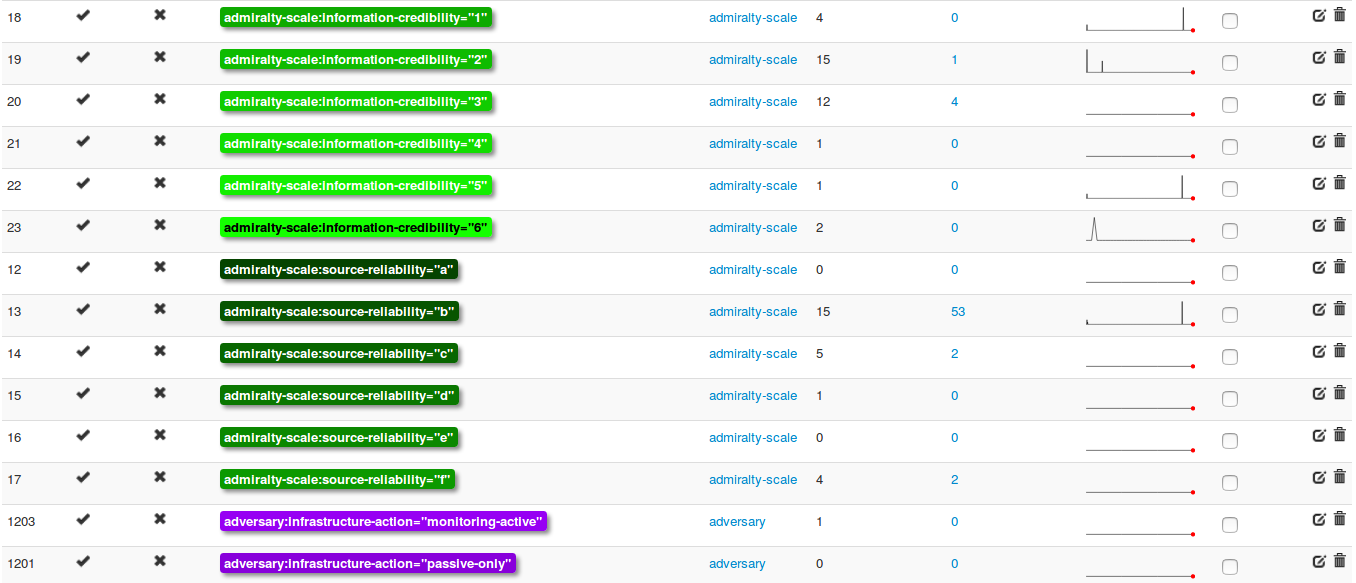
\includegraphics[scale=0.21]{tags-2-4-70.png}
\begin{itemize}
        \item MISP administrator can just import (or even cherry pick) the namespace or predicates they want to use as tags.
\item Tags can be exported to other instances.
\item Tags are also accessible via the MISP REST API.
\end{itemize}
\end{frame}


\begin{frame}
\frametitle{Filtering the distribution of events among MISP instances}
\begin{itemize}
\item Applying rules for distribution based on tags:
\end{itemize}
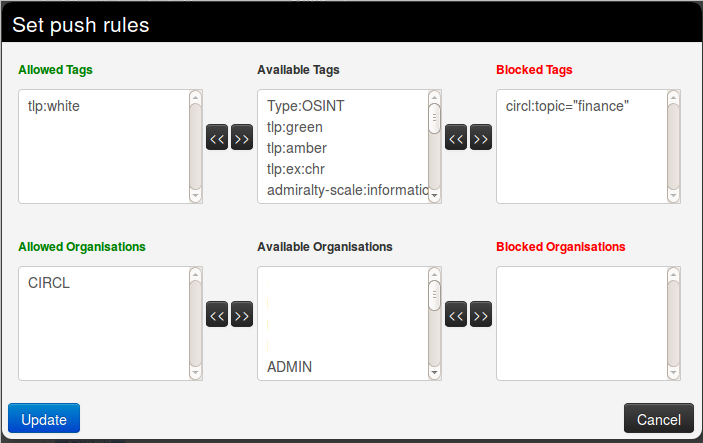
\includegraphics[scale=0.45]{tagspush.png}
\end{frame}

\begin{frame}
        \frametitle{Other use cases using MISP taxonomies}
\begin{itemize}
    \item Tags can be used to set events or attributes for {\bf further processing by external tools} (e.g. VirusTotal auto-expansion using Viper).
    \item Ensuring a classification manager {\bf classifies the events before release} (e.g. release of information from air-gapped/classified networks).
    \item {\bf Enriching IDS export} with tags to fit your NIDS deployment.
    \item Using {\bf IntelMQ} and MISP together to process events (tags limited per organization introduced in MISP 2.4.49).
\end{itemize}
\end{frame}

\begin{frame}
        \frametitle{Future functionalities related to MISP taxonomies}
\begin{itemize}
    \item {\bf Sighting} support (thanks to NCSC-NL) is integrated in MISP allowing to auto expire IOC based on user detection.
        \item Adjusting taxonomies (adding/removing tags) based on their score or visibility via sighting.
        \item Simple taxonomy editors to {\bf help non-technical users} to create their taxonomies.
        \item {\bf Filtering mechanisms} in MISP to rename or replace taxonomies/tags at pull and push synchronisation.
        \item More public taxonomies to be included.
\end{itemize}
\end{frame}

\begin{frame}
        \frametitle{PyTaxonomies}
\begin{itemize}
    \item {\bf Python module} to handle the taxonomies
    \item {\bf Offline} and online mode (fetch the newest taxonomies from GitHub)
    \item Simple {\bf search} to make tagging easy
        \item Totally independent from MISP
        \item {\bf No external dependencies} in offline mode
        \item Python3 only
        \item Can be used to create \& {\bf dump a new taxonomy}
\end{itemize}
\end{frame}

\begin{frame}[fragile]
        \frametitle{PyTaxonomies}
    \begin{lstlisting}[language=Python,basicstyle=\tiny]
from pytaxonomies import Taxonomies
taxonomies = Taxonomies()
taxonomies.version
# => '20160725'
taxonomies.description
# => 'Manifest file of MISP taxonomies available.'
list(taxonomies.keys())
# => ['tlp', 'eu-critical-sectors', 'de-vs', 'osint', 'circl', 'veris',
# 	  'ecsirt', 'dhs-ciip-sectors', 'fr-classif', 'misp', 'admiralty-scale', ...]
taxonomies.get('enisa').description
# 'The present threat taxonomy is an initial version that has been developed on
# the basis of available ENISA material. This material has been used as an ENISA-internal
# structuring aid for information collection and threat  consolidation purposes.
# It emerged in the time period 2012-2015.'
print(taxonomies.get('circl'))
# circl:incident-classification="vulnerability"
# circl:incident-classification="malware"
# circl:incident-classification="fastflux"
# circl:incident-classification="system-compromise"
# circl:incident-classification="sql-injection"
# ....
print(taxonomies.get('circl').machinetags_expanded())
# circl:incident-classification="Phishing"
# circl:incident-classification="Malware"
# circl:incident-classification="XSS"
# circl:incident-classification="Copyright issue"
# circl:incident-classification="Spam"
# circl:incident-classification="SQL Injection"

\end{lstlisting}
\end{frame}

\begin{frame}
        \frametitle{The dilemma of false-positives}
        \begin{itemize}
            \item False-positives are a {\bf common issue} in threat intelligence sharing.
                \item It's often a contextual issue:
                \begin{itemize}
                \item False-positives might be different per community of users sharing information.
                \item Organizations might have their {\bf own view} on false-positives.
                \end{itemize}
        \item Based on the success of the MISP taxonomy model, we built misp-warninglists.
        \end{itemize}
\end{frame}

\begin{frame}[t,fragile]
        \frametitle{MISP warning lists}
        \begin{itemize}
            \item misp-warninglists are lists of {\b well-known indicators} that can be associated to potential false positives, errors, or mistakes.
                \item Simple JSON files
        \end{itemize}
\begin{lstlisting}[language=json,firstnumber=1]
{
  "name": "List of known public DNS resolvers",
  "version": 2,
  "description": "Event contains one or more public DNS resolvers as attribute with an IDS flag set",
  "matching_attributes": [
    "ip-src",
    "ip-dst"
  ],
  "list": [
    "8.8.8.8",
    "8.8.4.4",...]
}
\end{lstlisting}
\end{frame}

\begin{frame}[t,fragile]
\frametitle{MISP warning lists}
\begin{itemize}
\item The warning lists are integrated in MISP to display an info/warning box at the event and attribute level.
\item Enforceable via the API where all attributes that have a hit on a warninglist will be excluded.
\item This can be enabled at MISP instance level.
\item Default warning lists can be enabled or disabled like {\bf known public resolver}, {\bf multicast IP addresses}, {\bf hashes for empty values}, {\bf rfc1918}, {\bf TLDs} or {\bf known Google domains}.
\item The warning lists can be expanded or added in JSON locally or via pull requests.
\item Warning lists can be also used for {\bf critical or core infrastructure warning}, {\bf personally identifiable information}...
\end{itemize}
\end{frame}


\begin{frame}[t,fragile] {Q\&A}

\includegraphics[scale=0.5]{misplogo.pdf}
\begin{itemize}
        \item \url{https://github.com/MISP/MISP}
        \item \url{https://github.com/MISP/misp-taxonomies}
        \item \url{https://github.com/MISP/PyTaxonomies}
        \item \url{https://github.com/MISP/misp-warninglists}
        \item info@circl.lu (if you want to join one of the MISP community operated by CIRCL)
        \item PGP key fingerprint: CA57 2205 C002 4E06 BA70 BE89 EAAD CFFC 22BD 4CD5
\end{itemize}

\end{frame}

